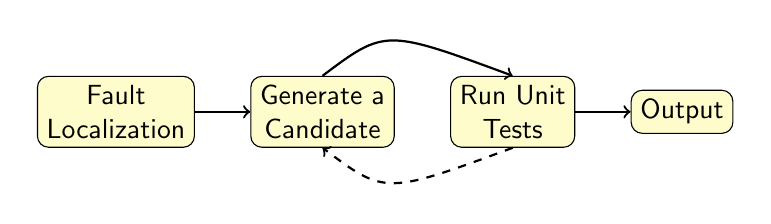
\begin{tikzpicture}[
  font=\sffamily,
  every matrix/.style={ampersand replacement=\&,column sep=2em,row sep=2em},
  box/.style={draw,rounded corners,fill=yellow!20},
  flow/.style={->, thick},
  fail/.style={->, thick, dashed},
  every node/.style={align=center}]
  
% Position the nodes using a matrix layout
\matrix{
      \node[box] (faultLocalization) {Fault \\ Localization};
      \& \node[box] (generateCandidate) {Generate a \\ Candidate};
      \& \node[box] (test) {Run Unit \\ Tests};
      \& \node[box] (output) {Output};
      \\
  };

% Draw the arrows between the nodes and label them.
\draw [flow] (faultLocalization) -- (generateCandidate);
\draw [flow] (generateCandidate.north) .. controls (up:3em) .. (test.north);
\draw [flow] (test) -- (output);
\draw [fail] (test.south) .. controls (down:3em) .. (generateCandidate.south);


% \draw [fail] (oracleInquisition.south) .. controls (down:.5em) and (left:8em) .. (oracleInquisition.west);
% \draw [fail] (collectionOfTestExecutionData) .. controls (down:2em) and (left:9em) .. (oracleInquisition.west);
% \draw [fail] (smtSolving.north) .. controls (down:2em) and (left:10em) .. (oracleInquisition.west);
\end{tikzpicture}
